\chapter{Hasil dan Pembahasan}
Bab ini akan menjelaskan hasil dari metode yang telah dijelaskan pada bab sebelumnya. 
Pembahasan akan dibagi berdasarkan fitur yang dikembangkan, dan akan menjelaskan mengenai hasil dari proses desain gamifikasi, hasil dari pengembangan aplikasi, dan proses pengujiannya masing-masing.
Selanjutnya dijelaskan juga mengenai pengujian keseluruhan aplikasi dengan melibatkan pengguna nyata atau responden.

\section{Hasil Pengembangan Desain Gamifikasi}
Gamifikasi yang diimplementasikan merupakan elemen gamifikasi untuk domain pembelajaran \textit{Declarative Knowledge}.
Dengan demikian elemen utama dari desain ini ialah pengembangan pemebalajaran yang akan diimplementasikan menjadi sebuah fitur materi yang disusun berurutan, dan sebuah kuis yang dapat dikerjakan berulang ulang.
Pengembangan gamifikasinya sendiri menggunakan \textit{Framework MDA} dimana kerangka kerja ini mengimplementasikan mekanika permainan, dinamika permainan, dan estetika permainan ke dalam aplikasi pembalajran ini.

Warna yang digunakan dalam desain aplikasi ini menggunakan warna utama hijau.
Hijau dipilih karena memberika kesan kesagaran dan kesehatan.
Pemilihan warna yang tepat untuk konteks pembelajaran merupakan upaya untuk memenuhi elemen estetika permainan untuk menarik pengguna menggunakan aplikasinya.  
Aplikasi ini dinamai "\textbf{MedQ}" untuk kesan \textit{simple} da mudah diingat. MedQ adalah kependekan dari \textit{Medical Education Quiz}.

Hasil pertama dari penelitain ini ialah \textit{prototype} desain \textit{Hi-fidelity wireframe} dari aplikasi yang akan dikembangkan.
\textit{Prototype} ini dibuat berdasarkan fitur set yang dikembangkan dan terdiri dari tema terang dan tema gelap. Setiap fitur set ini juga diidentifikasi apa saja elemen gamifikasi yang dapat diimplementasikan.
Setiap fitur set tentunya akan memiliki elemen dan tujuan gamifikasinya masing-masing. Dari \textit{prototype} yang dikembangkan, kemudian dibuat dalam bentuk aplikasi flutter sebagai \textit{front-end} untuk pengembangannya dengan \textit{back-end service} menggunakan \textit{firebase}.

% ===================================SIGN IN============================================================================================
\newpage
\subsection{\textit{Feature set: Sign-In}}
Set fitur yang pertama adalah sebuah halaman \textit{Sign-in} dimana pengguna akan mendaftarkan dirinya untuk dapat mengakses ke dalam aplikasi.
Cara pengguna melakukan \textit{Sign-in} ialah dengan menggunakan autentikasi akun \textit{Google}.
\begin{figure}[H]
	\centering
	\begin{subfigure}[b]{0.25\textwidth}
		\centering
	  
\includegraphics[width=\linewidth]{contents/chapter-3/images/HF-login.png}
	  \caption{\textit{Light Mode}}
	  \label{fig:HasilLogin}
	\end{subfigure}
	\begin{subfigure}[b]{0.25\textwidth}
		\centering
	  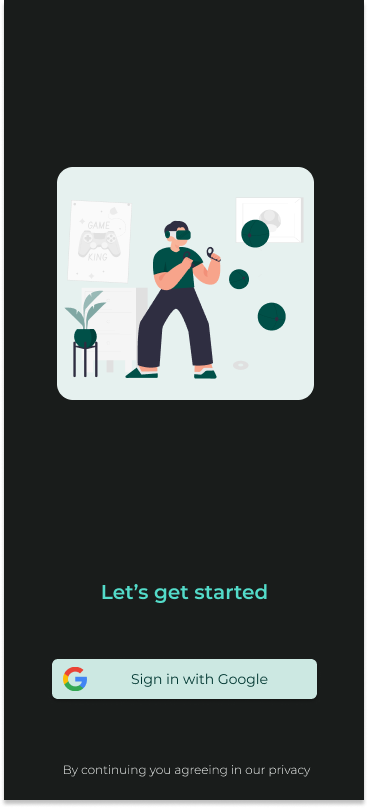
\includegraphics[width=\linewidth]{contents/chapter-3/images/HF-login-dt.png}
	  \caption{\textit{Dark Mode}}
	  \label{fig:HasilLogin2}
	\end{subfigure}
	\caption{\textit{Prototype} antarmuka halaman \textit{Sign-in}}
	\label{Fig:HasilFeatureSetLogin}
\end{figure}
Gambar \ref*{Fig:HasilFeatureSetLogin} merupakan \textit{prototype} dari halaman \textit{sign-in} aplikasi ini. 
Halaman ini menyediakan 1 tombol yang berfungsi untuk meminta autentikasi \textit{google} pada pengguna.
Gambar ditambahkan pada halaman ini untuk mendukung kesan estetika pada aplikasi. 
Serta ditambahkan juga tema gelap ke dalam aplikasi untuk mendapatkan kesan estetika ketika menggunakan mode gelap dalam \textit{handphone}.
\begin{table}[H]
	\caption{Tabel desain gamifikasi fitur \textit{Sign-in}}
	\begin{tabular}{|c|m{0.4\textwidth}|m{0.3\textwidth}|}
		\hline
		Elemen Gamifikasi& Letak Elemen & Tujuan Gamifikasi\\
		\hline
		\multirow{3}{2.5cm}{\textit{Aesthetic}}&\textit{User Interface}&Pengalaman pengguna yang menyenangkan\\
		\cline{2-3}
		& Tema gelap & Estetika modern dan kekinian \\
		\cline{2-3}
		& Gambar orang sedang bermain \textit{game} & Memberikan kesan estetika permainan pada pengguna \\
		\hline
	\end{tabular}
\end{table}
% ============================================
\subsection{\textit{Feature set: Dashboard}}
Fitur set selanjutnya ialah halaman \textit{On Boarding} yang didesain seperti pada gambar \ref*{Fig:HasilFeatureSetBoarding} dan \ref*{Fig:HasilFeatureSetBoarding-dt} . 
Halaman ini akan ditampilkan jika pengguna belum pernah \textit{Sign-in}. 
Tujuannya ialah memberikan kesan dinamika permainan yang akan ditempuh oleh penggunanya.
\begin{figure}[H]
	\centering
	\begin{subfigure}[b]{0.25\textwidth}
		\centering
	  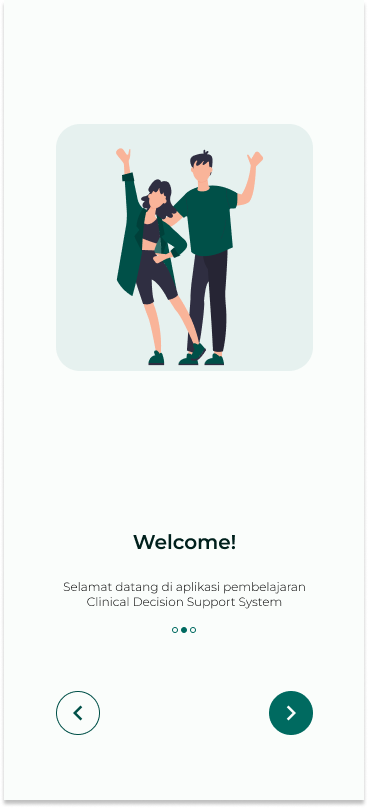
\includegraphics[width=\linewidth]{contents/chapter-3/images/HF-Boarding-1.png}
	  \caption{\textit{On Boarding (1)}}
	  \label{fig:HasilBoarding}
	\end{subfigure}
	\begin{subfigure}[b]{0.25\textwidth}
		\centering
	  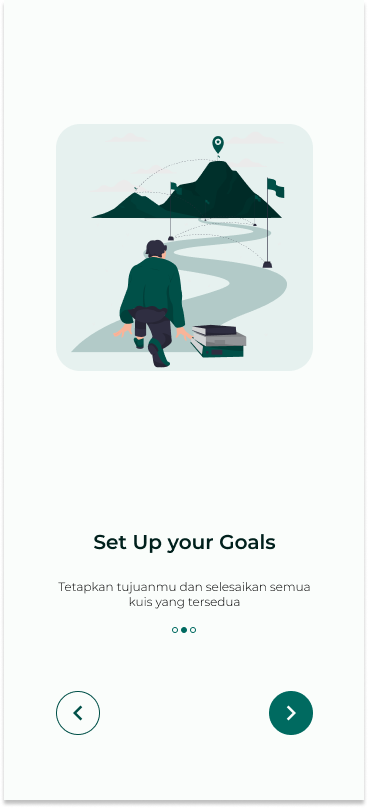
\includegraphics[width=\linewidth]{contents/chapter-3/images/HF-Boarding-2.png}
	  \caption{\textit{On Boarding (2)}}
	  \label{fig:HasilBoarding2}
	\end{subfigure}
	\begin{subfigure}[b]{0.25\textwidth}
		\centering
	  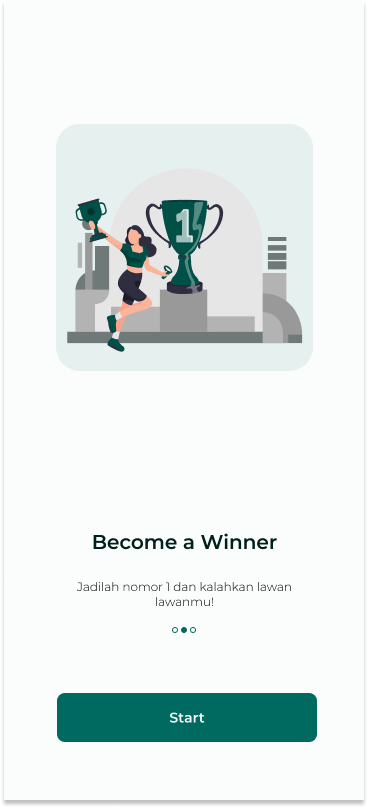
\includegraphics[width=\linewidth]{contents/chapter-3/images/HF-Boarding-3.png}
	  \caption{\textit{On Boarding (3)}}
	  \label{fig:HasilBoarding3}
	\end{subfigure}
	\caption{\textit{Prototype} antarmuka halaman \textit{On Boarding} tema terang}
	\label{Fig:HasilFeatureSetBoarding}
\end{figure}
\begin{figure}[H]
	\centering
	\begin{subfigure}[b]{0.25\textwidth}
		\centering
	  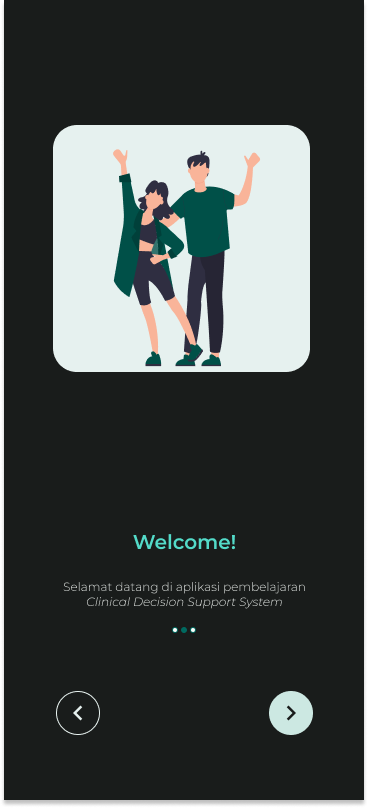
\includegraphics[width=\linewidth]{contents/chapter-3/images/HF-Boarding-1-dt.png}
	  \caption{\textit{On Boarding (1)}}
	  \label{fig:HasilBoarding1-dt}
	\end{subfigure}
	\begin{subfigure}[b]{0.25\textwidth}
		\centering
	  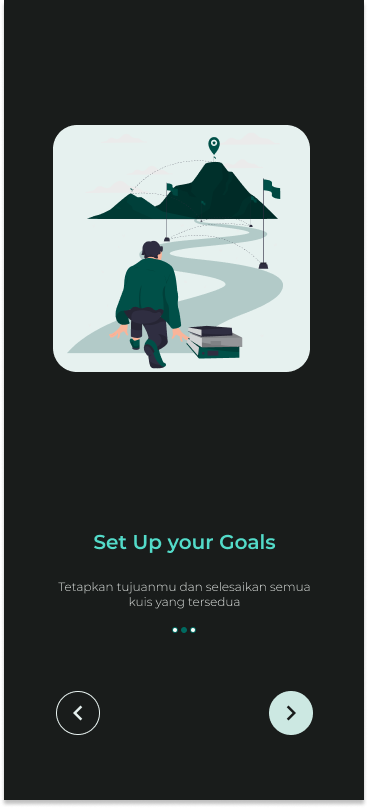
\includegraphics[width=\linewidth]{contents/chapter-3/images/HF-Boarding-2-dt.png}
	  \caption{\textit{On Boarding (2)}}
	  \label{fig:HasilBoarding2-dt}
	\end{subfigure}
	\begin{subfigure}[b]{0.25\textwidth}
		\centering
	  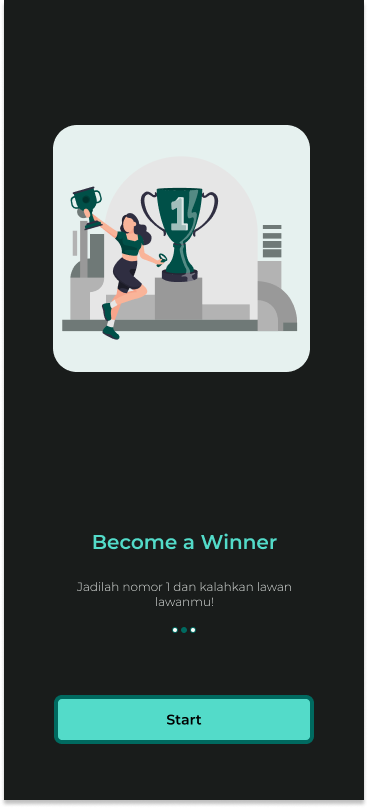
\includegraphics[width=\linewidth]{contents/chapter-3/images/HF-Boarding-3-dt.png}
	  \caption{\textit{On Boarding (3)}}
	  \label{fig:HasilBoarding3-dt}
	\end{subfigure}
	\caption{\textit{Prototype} antarmuka halaman \textit{On Boarding} tema gelap}
	\label{Fig:HasilFeatureSetBoarding-dt}
\end{figure}
Halaman \textit{on boarding} sendiri terdiri dari 3 halaman dengan kalimat yang berbeda tiap halamannya.
Tombol diberikan untuk berpindah halaman dan melanjutkan ke halaman \textit{Dashboard}.
\begin{table}[H]
	\caption{Tabel desain gamifikasi halaman \textit{on boarding}}
	\begin{tabular}{|p{3.6cm}|m{0.4\textwidth}|m{0.3\textwidth}|}
		\hline
		Elemen Gamifikasi& Letak Elemen & Tujuan Gamifikasi\\
		\hline
		\textit{Dynamic}&\textit{On boarding guide}&Memberikan informasi dinamika yang akan dilalui pengguna \\
		\hline
		\multirow{4}{1cm}{\textit{Aesthetic}}&\textit{User Interface}&Terlihat lebih menarik\\
		\cline{2-3}
		& Gambar orang sedang melambaikan tangan (Gambar \ref*{fig:HasilBoarding} dan \ref*{fig:HasilBoarding1-dt}) & Menunjukkan selamat datang pada pengguna \\
		\cline{2-3}
		& Gambar orang ingin memulai perjalanan dengan sebuah tujuan (Gambar \ref*{fig:HasilBoarding2} dan \ref*{fig:HasilBoarding2-dt}) & Menunjukkan salah satu dinamika permainan untuk menyelesaikan perjalanan yang perlu ditempuh \\
		\cline{2-3}
		& Gambar orang mendapatkan juara (Gambar \ref*{fig:HasilBoarding3} dan \ref*{fig:HasilBoarding3-dt}) & Menunjukkan salah satu dinamika permainan untuk mendapatkan skor tertinggi \\
		\hline
	\end{tabular}
\end{table}
Selain halaman \textit{On Boarding}, halaman utama aplikasi juga termasuk ke dalam fitur set ini. Desain halaman utama aplikasi ini terdapat pada gambar \ref*{Fig:HasilFeatureDashboard}.
Dalam halaman ini terdapat langsung 2 mode yang dimiliki oleh aplikasi ini. Kedua mode ini merupakan \textit{"rules"} atau mekanika permainan yang perlu diselesaikan oleh pengguna.
Mode tersebut terdiri dari mode materi dimana kita dapat melihat materi yang sudah disediakan dan mode kuis dimana kita akan mengujikan pengetahuan kita mengenai materi yang diberikan.
Kedua mode ini juga termasuk ke dalam dinamika permainan dimana pengguna dapat mendapatkan materi dan menguji coba kuis yang disediakan.
Halaman ini juga dapat menampilkan \textit{side drawer} untuk melihat profil dan juga tombol untuk \textit{sign-out} dari aplikasi.
\textit{Side drawer} ini juga mampu menampilkan \textit{tab-tab} lain yang dapat diatur navigasinya. Untuk penelitian ini \textit{tab} tersebut hanya diisi oleh informasi pengembang dan media sosial pengembang.

\begin{figure}[H]
	\centering
	\begin{subfigure}[b]{0.24\textwidth}
		\centering
	  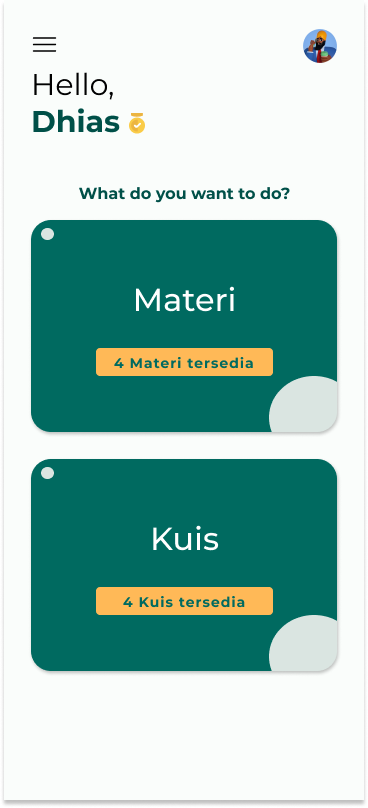
\includegraphics[width=\linewidth]{contents/chapter-3/images/HF-Main.png}
	  \caption{Halaman utama}
	  \label{fig:HasilMainDash}
	\end{subfigure}
	\begin{subfigure}[b]{0.24\textwidth}
		\centering
	  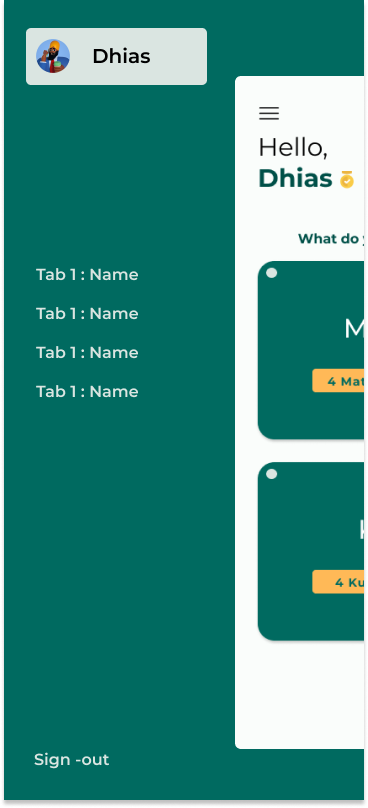
\includegraphics[width=\linewidth]{contents/chapter-3/images/HF-Drawer.png}
	  \caption{\textit{Drawer}}
	  \label{fig:HasilMainDash2}
	\end{subfigure}
	\begin{subfigure}[b]{0.24\textwidth}
		\centering
	  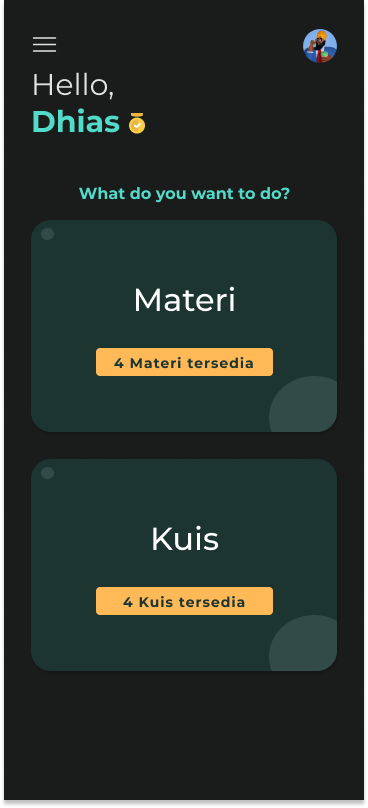
\includegraphics[width=\linewidth]{contents/chapter-3/images/HF-Main-dt.png}
	  \caption{Halaman Utama}
	  \label{fig:HasilMainDash-dark}
	\end{subfigure}
    \begin{subfigure}[b]{0.24\textwidth}
		\centering
	  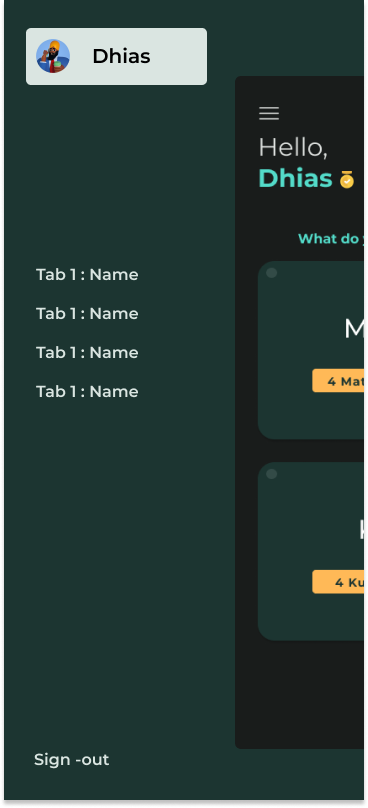
\includegraphics[width=\linewidth]{contents/chapter-3/images/HF-Drawer-dt.png}
	  \caption{\textit{Drawer}}
	  \label{fig:HasilMainDash2-dark}
	\end{subfigure}
	\caption{\textit{Prototype} antarmuka halaman \textit{Dashboard} utama}
	\label{Fig:HasilFeatureDashboard}
\end{figure} 

\begin{table}[H]
	\caption{Tabel desain gamifikasi halaman \textit{Dashboard}}
	\begin{tabular}{|m{3.6cm}|m{0.4\textwidth}|m{0.3\textwidth}|}
		\hline
		Elemen Gamifikasi& Letak Elemen & Tujuan Gamifikasi\\
		\hline
		\textit{Mechanic}&\textit{Mode}& Diberikan mode sebagai mekanika yang  dapat dikerjakan oleh pengguna \\
		\hline
		\multirow{3}{1cm}{\textit{Aesthetic}}&\textit{User Interface}&Pengalaman pengguna yang menyenangkan\\
		\cline{2-3}
		& Tema gelap & Estetika modern dan kekinian \\
		\cline{2-3}
		& Foto profil & Estetika menunjukkan pemilik akun \\
		\hline
	\end{tabular}
\end{table}
\subsection{\textit{Feature set: Quiz}}
Fitur set selanjutnya ilah fitur set aktivitas mengerjakan kuis. 
Desain yang pertama dibuat ialah desain untuk memilih kuis yang akan dikerjakan seperti tergambar pada gambar \ref*{Fig:HasilFeatureSetQuizListt}.
Pada gambar tersebut disajikan daftar kuis yang tersedia pada aplikasi.
Masing-masing daftar akan membuka halaman kuis yang terdapat pada gambar \ref*{Fig:HasilFeatureSetQuiz}.
Masing-masing daftar tersebut juga terdapat tombol untuk menuju halaman fitur set \textit{leaderboard}.
Kuis tersebut sengaja disajikan berurutan untuk memberikan kesan dinamika permainan dalam aplikasi ini.
\begin{figure}[H]
	\centering
	\begin{subfigure}[b]{0.3\textwidth}
		\centering
	  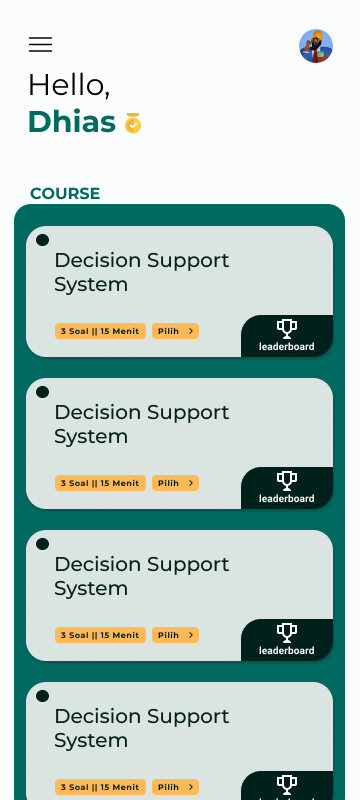
\includegraphics[width=\linewidth]{contents/chapter-3/images/HF-QuizList.png}
	  \caption{\textit{Light Mode}}
	  \label{fig:HasilQuizList}
	\end{subfigure}
	\begin{subfigure}[b]{0.3\textwidth}
		\centering
	  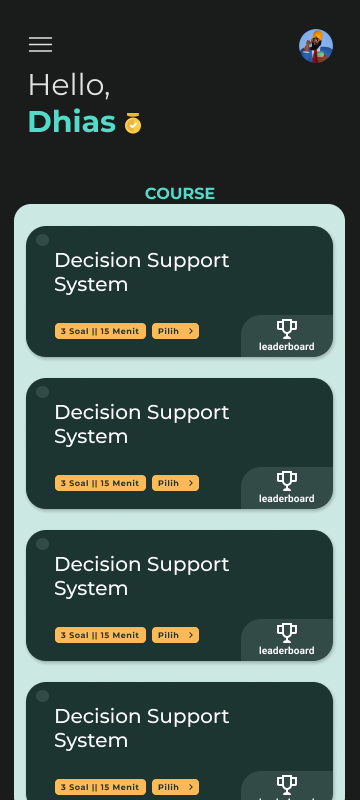
\includegraphics[width=\linewidth]{contents/chapter-3/images/HF-QuizList-dt.png}
	  \caption{\textit{Dark Mode}}
	  \label{fig:HasilQuizList2}
	\end{subfigure}
	\caption{\textit{Prototype} antarmuka halaman daftar kuis}
	\label{Fig:HasilFeatureSetQuizListt}
\end{figure}
Gambar \ref*{Fig:HasilFeatureSetQuizListt} merupakan halaman utama ketika pengguna memasuki mode kuis. Mode kuis ini akan menampilkan daftar kuis yang tersedia sebagai pilihan bagi pengguna mengenai kuis yang akan dikerjakan.
Elemen gamifikasi dalam halaman ini dijelaskan secara rinci pada Tabel \ref*{TabelGameDaftarKuis}.
\begin{table}[H]
	\caption{Tabel desain gamifikasi halaman daftar kuis}
	\label{TabelGameDaftarKuis}
	\begin{tabular}{|m{3.6cm}|m{0.4\textwidth}|m{0.3\textwidth}|}
		\hline
		Elemen Gamifikasi& Letak Elemen & Tujuan Gamifikasi\\
		\hline
		\multirow{3}{1cm}{\textit{Mechanic}}&Informasi mengenai jumlah soal dan waktu pengerjaan& Memberikan aturan dalam pengerjaan soal\\
		\cline{2-3}
		&Navigasi fitur \textit{Leaderboard}&Meberikan pengalaman kompetitif pada penggnua\\
		\hline
		\textit{Dynamic}&Materi berurutan&Memberikan pengalaman belajar secara berurutan \\
		\hline
		\multirow{3}{1cm}{\textit{Aesthetic}}&\textit{User Interface}&Terlihat lebih menarik\\
		\cline{2-3}
		& Tema gelap & Estetika modern dan kekinian \\
		\hline
	\end{tabular}
\end{table}
\newpage
Selanjutnya halaman daftar kuis pada Gambar \ref*{Fig:FeatureSetQuiz}.
Halaman kuis ini terdiri dari halaman menjawab kuis, melihat \textit{overview} kuis, dan mensubmit kuis.
\begin{figure}[H]
	\centering
	\begin{subfigure}[b]{0.23\textwidth}
		\centering
	  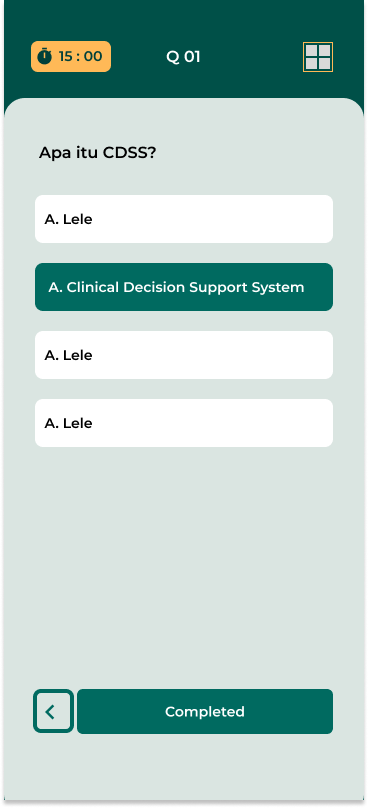
\includegraphics[width=\linewidth]{contents/chapter-3/images/HF-kuis1.png}
	  \caption{Jawab kuis}
	  \label{fig:midFi-login}
	\end{subfigure}
	\begin{subfigure}[b]{0.23\textwidth}
		\centering
	  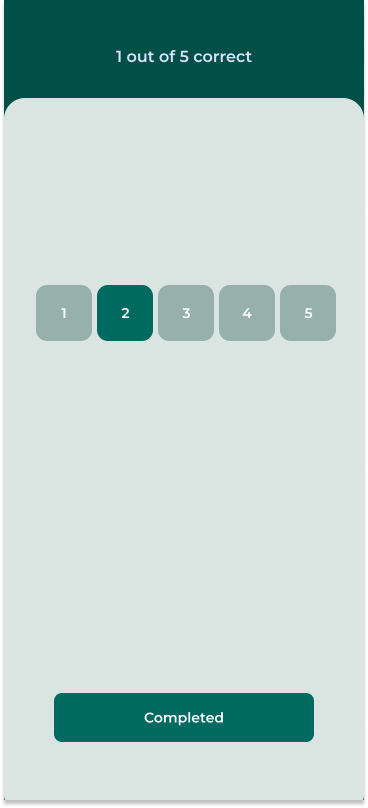
\includegraphics[width=\linewidth]{contents/chapter-3/images/HF-kuis2.png}
	  \caption{\textit{overview}}
	  \label{fig:pilihNomor}
	\end{subfigure}
	\begin{subfigure}[b]{0.23\textwidth}
		\centering
	  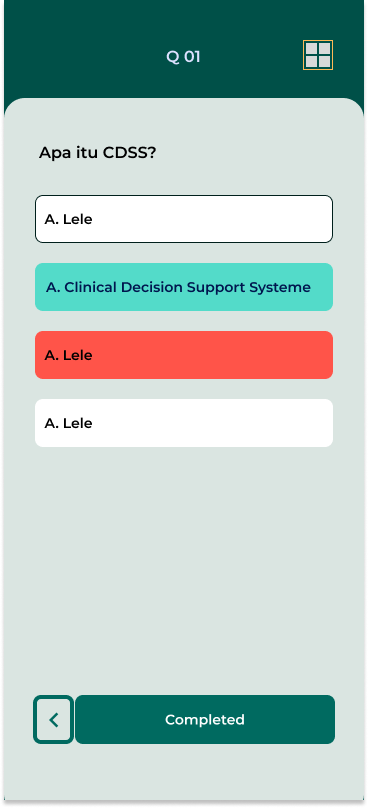
\includegraphics[width=\linewidth]{contents/chapter-3/images/HF-kuis3.png}
	  \caption{\textit{Review}}
	  \label{fig:subjectScreen}
	\end{subfigure}
	\caption{\textit{Prototype} antarmuka halaman kuis tema terang}
	\label{Fig:HasilFeatureSetQuiz}
\end{figure}
Pada halaman ini mekanika permainan yang diberikan ialah waktu yang menentukan berapa lama kuis tersebut dikerjakan.
Elemen waktu ini juga dapat menjadi dinamika permainan karena akan memperngaruhi respon pengguna saat mengerjakan kuis.
Fitur set ini juga yang menentukan mekanika permainan poin yang akan didapatkan oleh pengguna. Semakin banyak jawaban yang benar dan waktu yang cepat, semakin besar juga poin yang akan didapatkan.
\begin{figure}[H]
	\centering
	\begin{subfigure}[b]{0.23\textwidth}
		\centering
	  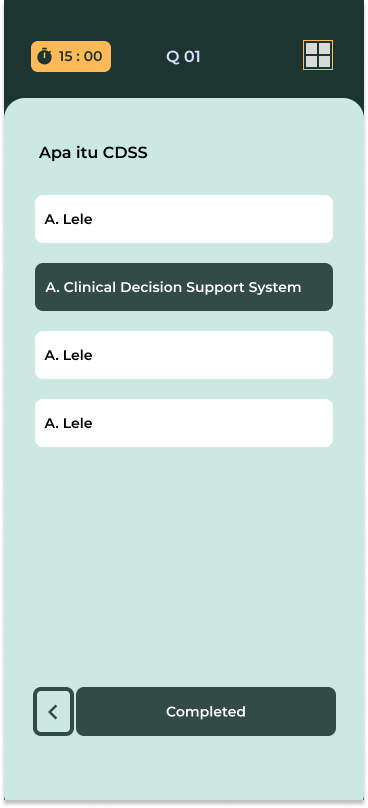
\includegraphics[width=\linewidth]{contents/chapter-3/images/HF-kuis1-dt.png}
	  \caption{Jawab kuis}
	  \label{fig:pilihJawabanDark}
	\end{subfigure}
	\begin{subfigure}[b]{0.23\textwidth}
		\centering
	  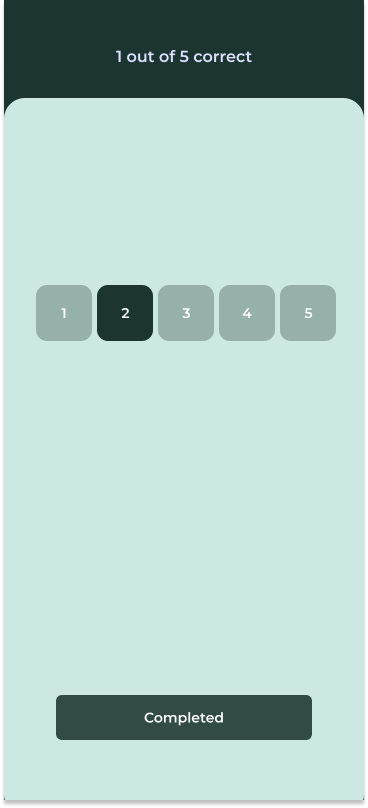
\includegraphics[width=\linewidth]{contents/chapter-3/images/HF-kuis2-dt.png}
	  \caption{\textit{Overview}}
	  \label{fig:pilihNomorDark}
	\end{subfigure}
	\begin{subfigure}[b]{0.23\textwidth}
		\centering
	  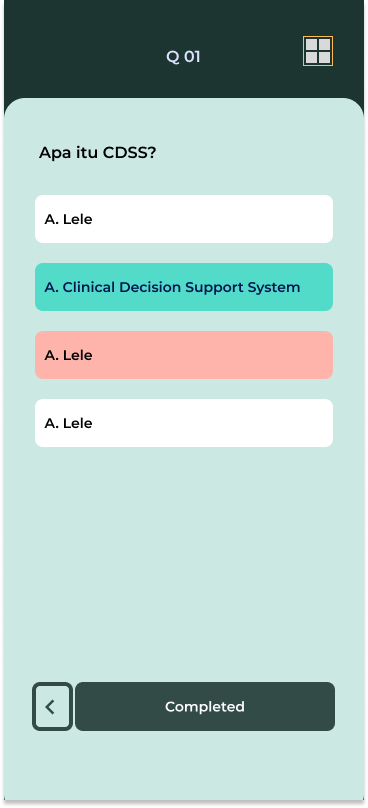
\includegraphics[width=\linewidth]{contents/chapter-3/images/HF-kuis3-dt.png}
	  \caption{\textit{Review}}
	  \label{fig:KoreksiDark}
	\end{subfigure}
	\caption{\textit{Prototype} antarmuka halaman kuis tema gelap}
	\label{Fig:FeatureSetQuizDark}
\end{figure}
\begin{table}[H]
	\caption{Tabel desain gamifikasi halaman pengerjaan kuis}
	\label{TabelGameIsiKuis}
	\begin{tabular}{|m{3.6cm}|m{0.4\textwidth}|m{0.3\textwidth}|}
		\hline
		Elemen Gamifikasi& Letak Elemen & Tujuan Gamifikasi\\
		\hline
		\multirow{3}{1cm}{\textit{Mechanic}}&Pengerjaan Kuis& Aturan utama dalam fitur kuis bagi pengguna\\
		\cline{2-3}
		&Navigasi nomor kuis&Meberikan keleluasaan bagi pengguna untuk mengerjakan soal\\
		\cline{2-3}
		&\textit{Time Attack}& Memberikan kesan adrenalin pengerjaan kuis\\
		\cline{2-3}
		&\textit{Overview}& Memberikan akses melompati soal\\
		\hline
		\textit{Dynamic}&Soal&Memberikan pengalaman belajar secara berurutan \\
		\hline
		\multirow{3}{1cm}{\textit{Aesthetic}}&\textit{User Interface}&Terlihat lebih menarik\\
		\cline{2-3}
		& Tema gelap & Estetika modern dan kekinian \\
		\cline{2-3}
		&\textit{Highlight} jawaban benar dan salah& Memberikan visual yang berbeda anatara jawaban yang benar dan yang salah\\
		\cline{2-3}
		&\textit{Highlight} jawaban yang belum diisi dan yang sudah& Memberikan visual yang berbeda anatara jawaban yang diisi dan yang belum diisi\\
		\hline
	\end{tabular}
\end{table}
Untuk estetika pada fitur ini sama halnya pada keseluruhan aplikasi, terdapat 2 tema yang akan mengikuti tema pada sistem android.
Tema terang fitur ini terdapa pada gambar \ref*{Fig:HasilFeatureSetQuiz}, sedagkan tema gelap terdapat pada gambar \ref*{Fig:FeatureSetQuizDark}.

Fitur set ini ditutup dengan hasil yang akan didapatkan pengguna setelah mengerjakan kuis. Poin benar akan langsung dihitung dan dikirimkan pada \textit{database} aplikasi.
Poin tersebut kemudian diurutkan berdasarkan poin tertinggi pada kuis terkait. Halaman hasil ditampilkan pada gambar \ref*{Fig:HasilFeatureSetQuizResult}
\begin{figure}[H]
	\centering
	\begin{subfigure}[b]{0.23\textwidth}
		\centering
	  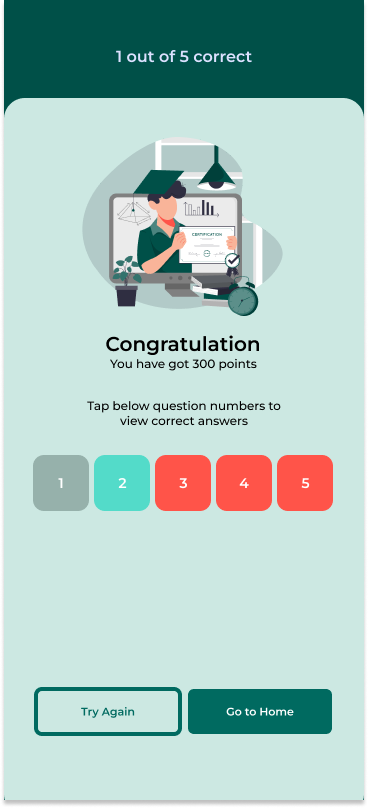
\includegraphics[width=\linewidth]{contents/chapter-3/images/HF-result.png}
	  \caption{\textit{Light Mode}}
	  \label{fig:HasilQuizResult}
	\end{subfigure}
	\begin{subfigure}[b]{0.23\textwidth}
		\centering
	  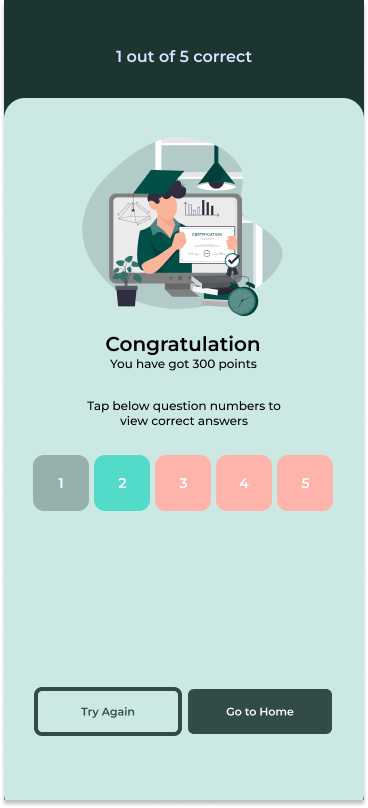
\includegraphics[width=\linewidth]{contents/chapter-3/images/HF-result-dt.png}
	  \caption{\textit{Dark Mode}}
	  \label{fig:HasilQuizResult2}
	\end{subfigure}
	\caption{\textit{Prototype} antarmuka halaman hasil kuis}
	\label{Fig:HasilFeatureSetQuizResult}
\end{figure}
Halaman hasil ini akan menampilkan poin yang diperoleh oleh pengguna dan jumlah jawaban yang benar dijawab oleh pengguna.
Elemen gamifikasi yang diimplementasikan diantara dirangkum pada Tabel\ref*{TabelGameHasilKuis}
\begin{table}[H]
	\caption{Tabel desain gamifikasi halaman hasil kuis}
	\label{TabelGameHasilKuis}
	\begin{tabular}{|m{3.6cm}|m{0.35\textwidth}|m{0.4\textwidth}|}
		\hline
		Elemen Gamifikasi& Letak Elemen & Tujuan Gamifikasi\\
		\hline
		\multirow{3}{1cm}{\textit{Mechanic}}&Kembali ke halaman utama& Memberikan akses untuk kembali ke mode utama atau halaman utama\\
		\cline{2-3}
		&\textit{Time}& Memberikan total waktu pengerjaan yang telah dilakukan\\
		\cline{2-3}
		&\textit{Overview}& Memberikan akses melihat hasil soal\\
		\hline
		\textit{Dynamic}&Pilihan mengulangi pengerjaan&Memberikan repetisi pembelajaran kepada pengguna \\
		\hline
		\multirow{3}{1cm}{\textit{Aesthetic}}&\textit{User Interface}&Terlihat lebih menarik\\
		\cline{2-3}
		& Tema gelap & Estetika modern dan kekinian \\
		\cline{2-3}
		&\textit{Highlight} jawaban benar dan salah& Memberikan visual yang berbeda anatara jawaban yang benar dan yang salah\\
		\cline{2-3}
		& Gambar penghargaan& Memberikan kesan penghargaan yang dicapai pengguna\\
		\hline
	\end{tabular}
\end{table}
\subsection{\textit{Feature set}: Materi}
Desain selanjutnya ialah halaman untuk fitur materi. Gambar \ref*{Fig:HasilFeatureSetDrawer} adalah desain dari fitur set materi yang
dapat menampilkan materi dalam bentuk .pdf dan dapat diakses secara berurutan.
Hal ini merupakan dinamika permaianan yang diterapkan pada aplikasi ini.
\begin{figure}[H]
	\centering
	\begin{subfigure}[b]{0.23\textwidth}
		\centering
	  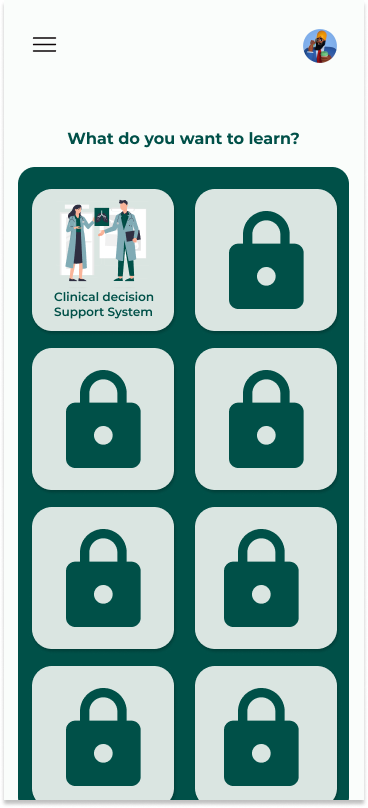
\includegraphics[width=\linewidth]{contents/chapter-3/images/HF-materi.png}
	  \caption{Daftar materi}
	  \label{fig:HasilMain2}
	\end{subfigure}
	\begin{subfigure}[b]{0.23\textwidth}
		\centering
	  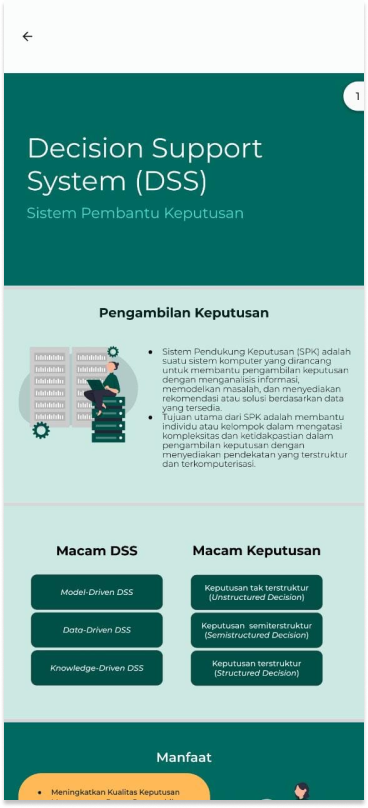
\includegraphics[width=\linewidth]{contents/chapter-3/images/HF-materi2.png}
	  \caption{Materi}
	  \label{fig:HasilMain3}
	\end{subfigure}
	\begin{subfigure}[b]{0.23\textwidth}
		\centering
	  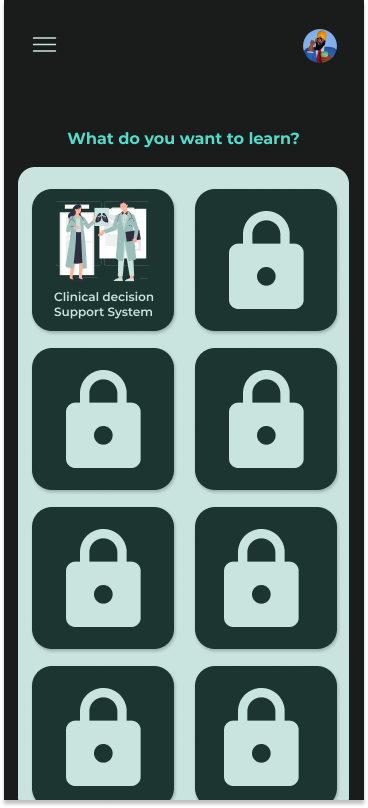
\includegraphics[width=\linewidth]{contents/chapter-3/images/HF-materi-dt.png}
	  \caption{Daftar materi}
	  \label{fig:HasilMain4-dark}
	\end{subfigure}
    \begin{subfigure}[b]{0.23\textwidth}
		\centering
	  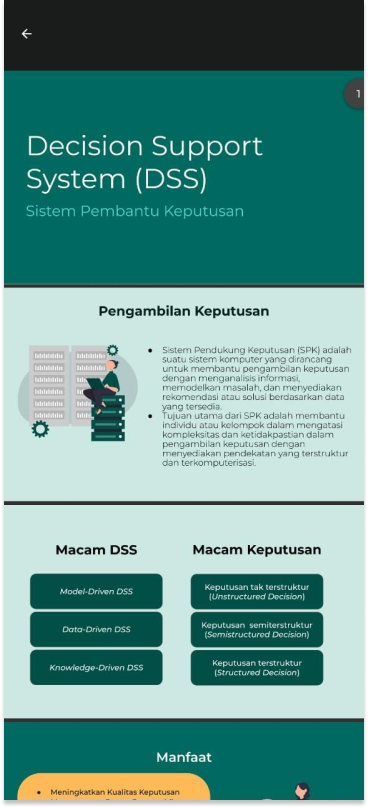
\includegraphics[width=\linewidth]{contents/chapter-3/images/HF-materi2-dt.png}
	  \caption{Materi}
	  \label{fig:HasilMain4}
	\end{subfigure}
	\caption{\textit{Prototype} antarmuka halaman fitur materi}
	\label{Fig:HasilFeatureSetDrawer}
\end{figure}
\begin{table}[H]
	\caption{Tabel desain gamifikasi halaman fitur materi}
	\label{TabelGameMateri}
	\begin{tabular}{|m{3.6cm}|m{0.35\textwidth}|m{0.4\textwidth}|}
		\hline
		Elemen Gamifikasi& Letak Elemen & Tujuan Gamifikasi\\
		\hline
		\textit{Mechanic}&Memilih materi& Memiliki keleluasaan jika ingin mengakses ulang materi\\
		\hline
		\textit{Dynamic}&Mempelajari materi secara berurutan&Memberikan pengalaman belajar yang berurutan \\
		\hline
		\multirow{3}{1cm}{\textit{Aesthetic}}&\textit{User Interface}&Terlihat lebih menarik\\
		\cline{2-3}
		& Tema gelap & Estetika modern dan kekinian \\
		\cline{2-3}
		&Gambar ilustrasi& Memberikan ilustrasi visual sesuai dengan materi\\
		\hline
	\end{tabular}
\end{table}
Fitur ini dibuat seperti demikian bertujuan untuk meningkatkan \textit{Engagement} kognitif dimana pengguna yang terlibat secara kognitif aktif dalam memproses, menganalisis, dan menafsirkan informasi secara terurut.
\subsection{\textit{Feature set: Leaderboard}}
Fitur set selanjutnya ialah \textit{Leaderboard}. Pada Gambar \ref*{Fig:HasilFeatureSetLeaderboard} merupakan desain hasil halaman \textit{Leaderboard} pada mode terang dan mode gelap.
Fitur ini merupakan salah satu fitur yang diharapkan masuk ke dalam aspek \textit{Social Student Engagement} yang diimplementasikan ke dalam aplikasi MedQ.
\begin{figure}[H]
	\centering
	\begin{subfigure}[b]{0.26\textwidth}
		\centering
	  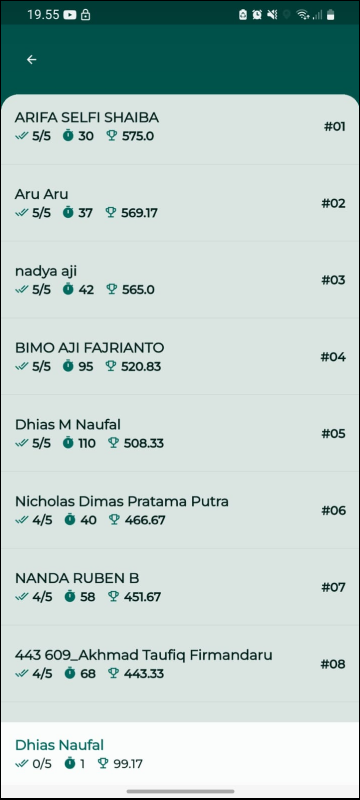
\includegraphics[width=\linewidth]{contents/chapter-3/images/HF-Leaderboard.png}
	  \caption{\textit{Light Mode}}
	  \label{fig:HasilQuizLeader}
	\end{subfigure}
	\begin{subfigure}[b]{0.26\textwidth}
		\centering
	  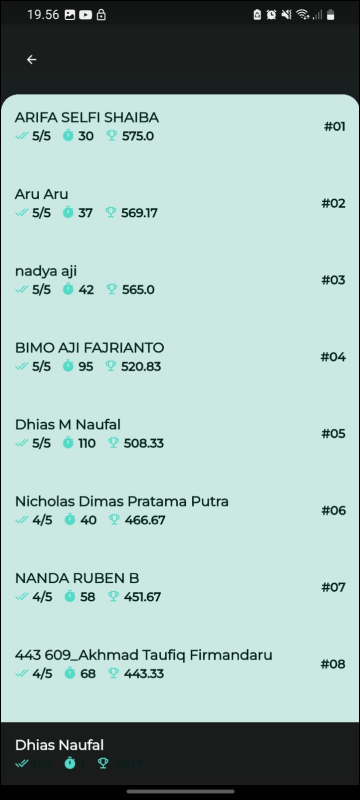
\includegraphics[width=\linewidth]{contents/chapter-3/images/HF-Leaderboard-dt.png}
	  \caption{\textit{Dark Mode}}
	  \label{fig:HasilQuizLeader2}
	\end{subfigure}
	\caption{\textit{Prototype} antarmuka halaman \textit{Leaderboard}}
	\label{Fig:HasilFeatureSetLeaderboard}
\end{figure}
Fitur \textit{Leaderboard} ini akan mengurutkan poin pengguna yang telah didapatkan pada fitur set kuis.
Pengguna akan berlomba mendapatkan urutan pertama dalam fitur ini dan akan meningkatkan \textit{social engagement} bagi pengguna
Halaman ini akan mengambil semua data poin yang sudah dikerjakan oleh penggunanya dan diurutkan berdasarkan point tertinggi.
Fitur ini juga merupakan salah satu elemen dinamika yang diimplementasikan dalam aplikas.
\begin{table}[H]
	\caption{Tabel desain gamifikasi halaman \textit{Leaderboard}}
	\label{TabelGameLeaderboard}
	\begin{tabular}{|m{3.6cm}|m{0.35\textwidth}|m{0.4\textwidth}|}
		\hline
		Elemen Gamifikasi& Letak Elemen & Tujuan Gamifikasi\\
		\hline
		\textit{Dynamic}&Urutan poin tertinggi&Memberikan pengalaman kompetitif bagi pengguna \\
		\hline
		\multirow{2}{1cm}{\textit{Aesthetic}}&\textit{User Interface}&Terlihat lebih menarik\\
		\cline{2-3}
		& Tema gelap & Estetika modern dan kekinian \\
		\hline
	\end{tabular}
\end{table}
\subsection{\textit{Feature set: Achievement}}
Kuis yang sudah dikerjakan akan terdaftar pada halaman profil. Daftar ini sama halnya dengan \textit{Achievement} yang didapat ketika pengguna selesai mengerjakannya.
\begin{figure}[H]
	\centering
	\begin{subfigure}[b]{0.23\textwidth}
		\centering
	  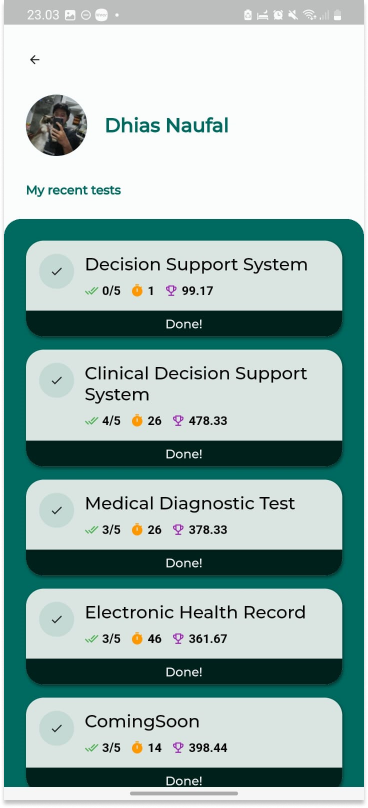
\includegraphics[width=\linewidth]{contents/chapter-3/images/HF-profil.png}
	  \caption{\textit{Light Mode}}
	  \label{fig:HasilQuizprofil}
	\end{subfigure}
	\begin{subfigure}[b]{0.23\textwidth}
		\centering
	  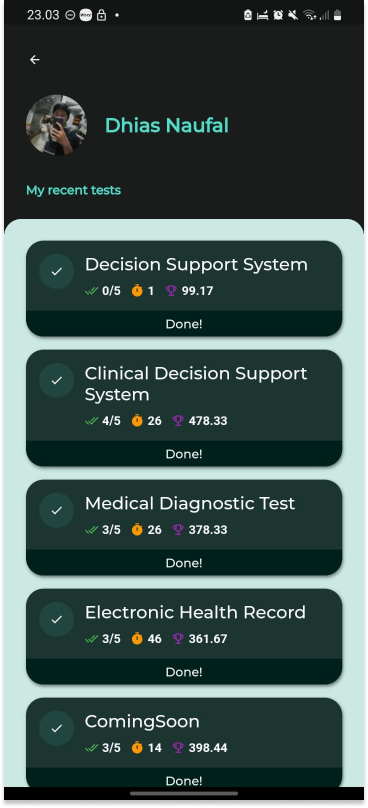
\includegraphics[width=\linewidth]{contents/chapter-3/images/HF-profil-dt.png}
	  \caption{\textit{Dark Mode}}
	  \label{fig:HasilQuizprofil2}
	\end{subfigure}
	\caption{\textit{Prototype} antarmuka halaman \textit{profile}}
	\label{Fig:HasilFeatureSetProfil}
\end{figure}
Gambar \ref*{Fig:HasilFeatureSetProfil} adalah desain halaman profil pada mode terang dan mode gelap. Fitur ini merupakan elemen mekanika permaianan dimana pengguna akan mendapatkan penghargaan sebanyak banyaknya.
Hal ini juga akan mempengaruhi dinamika permainan dimana pengguna akan berlomba dengan pengguna lain untuk mendapatkan lebih banyak penghargaan. 
\begin{table}[H]
	\caption{Tabel desain gamifikasi halaman \textit{Achievement}}
	\label{TabelGameAchivement}
	\begin{tabular}{|m{3.6cm}|m{0.35\textwidth}|m{0.4\textwidth}|}
		\hline
		Elemen Gamifikasi& Letak Elemen & Tujuan Gamifikasi\\
		\hline
		\textit{Mechanic}&\textit{Badge} Penghargaam &Memberikan motivasi untuk mengumpulkan penghargaan sebanyak banyaknya \\
		\hline
		\multirow{2}{1cm}{\textit{Aesthetic}}&\textit{User Interface}&Terlihat lebih menarik\\
		\cline{2-3}
		& Tema gelap & Estetika modern dan kekinian \\
		\hline
	\end{tabular}
\end{table}


\section{Hasil Pengembangan Aplikasi}
Proses pengembangan aplikasi ini menggunakan pendekatan \textit{FDD} dimana aplikasi akan dikembangakan berdasarkan fitur yang sudah didesain.
Aplikasi yang dikembangkan ialah aplikasi \textit{android} dengan menggunakan \textit{software development kit flutter} sebagai kerangka kerjanya.
Hasil pengembangan ini memiliki indikator keberhasilan melalui pengujian fungsionalitas dari setiap fiturnya.
\subsection{Fitur \textit{Sign-in} dan \textit{Sign-out}}
Fitur yang pertama dilakukan pengujian ialah fitur \textit{Sign-in} dan \textit{Sign-out}. Pengujian ini dilakaukan pertama untuk memastikan apakah pengguna bisa mengakses aplikasi dan dapat dicatat pada \textit{database}.
\begin{table}[H]
	\centering
	\caption{\textit{Black Box Testing} fitur \textit{Sign-in} dan \textit{Sign-out}}
	\label{Tab:blackBoxSign}
	\begin{tabular}{|p{0.4\textwidth}|p{0.4\textwidth}|p{0.1\textwidth}|}
		\hline
		 \centering\textbf{Fitur} & \multicolumn{1}{m{0.45\textwidth}|}{\centering \textbf{Kriteria}}&  \multicolumn{1}{m{0.1\textwidth}|}{\centering \textbf{Hasil}}\\
		\hline
		Menampilkan halaman Sign-in 
		& Aplikasi mampu menampilkan halaman \textit{sign-in} 
		& Berhasil\\
		\hline
		Mencatat \textit{user} baru ketika melakukan \textit{Sign-in} pertama 
		& Aplikasi dapat mencatat \textit{user} baru ketika melakukan \textit{Sign-in} pertama dan mengirimkannya ke \textit{database}
		& Berhasil\\
		\hline
		Aplikasi dapat memberikan akses pengguna ketika pengguna sudah terdaftar
		& Pengguna dapat menggunakan fitur aplikasi
		& Berhasil\\
		\hline
		Menghentikan pemberian akses pengguna ketika pengguna sudah terdaftar
		& Aplikasi mampu mengeluarkan akses aplikasi apda akun terkait
		& Berhasil\\
		\hline
	\end{tabular}
\end{table}
Pengujian fitur \textit{Sign-in} dan \textit{Sign-out} memiliki 4 aktivitas pengujian yang terdapat pada tabel \ref*{Tab:blackBoxSign}.
Pengujian ini medaparkan hasil 100\% berhasil untuk setiap aktivitas pengujiannya. Pengujian dilakukan dengan menggunakan beberapa \textit{device} untuk mendapatkan hasil yang lebih baik.
\newpage
\subsection{Fitur \textit{Dashboard}}
Pengujian selanjutnya ialah fitur \textit{Dashboard}. Halaman fitur ini dikembangkan pertama kali karena merupakan fitur \textit{"root"} dalam aplikasi ini.
\begin{table}[H]
	\centering
	\caption{\textit{Black Box Testing} fitur \textit{Dashboard}}
	\label{Tab:blackBoxDash}
	\begin{tabular}{|p{0.4\textwidth}|p{0.4\textwidth}|p{0.1\textwidth}|}
		\hline
		 \centering\textbf{Fitur} & \multicolumn{1}{m{0.45\textwidth}|}{\centering \textbf{Kriteria}}&  \multicolumn{1}{m{0.1\textwidth}|}{\centering \textbf{Hasil}}\\
		\hline
		Menampilkan halaman \textit{On Boarding} jika \textit{user} belum terdaftar 
		& Aplikasi mampu menampilkan halaman \textit{On Boarding} jika \textit{user} belum terdaftar  
		& Berhasil\\
		\hline
		Menampilkan halaman utama aplikasi
		& Ketika sudah \textit{sign-in}, penguna dapat mengakses halalman utama 
		& Berhasil\\
		\hline
		Menampilkan \textit{side drawer}
		& Aplikasi mempu menampilkan \textit{side drawer} pada sebelah kiri aplikasi
		& Berhasil\\
		\hline
		\textit{Dialog box Sign Up} jika memilih fitur, tapi \textit{user} belum terdaftar
		& Jika pengguna belum \textit{sign-in}, aplikasi menampilkan dialog box 
		& Berhasil\\
		\hline
		Memilih fitur kuis, materi, dan profil
		& Aplikasi mampu menampilkan semua fitur yang ada
		& Berhasil\\
		\hline
	\end{tabular}
\end{table}
Pengujian fitur \textit{Dashboard} memiliki 5 aktivitas pengujian yang terdapat pada tabel \ref*{Tab:blackBoxDash}.
Pengujian ini medaparkan hasil 100\% berhasil untuk setiap aktivitas pengujiannya. Pengujian ini dilakukan berulang-ulang untuk memastikan semua fitur dapat berjalan.
\newpage
\subsection{Fitur \textit{Quiz}}
Pengujian dilanjutkan dengan pepngujian fitur set kuis. Fitur set kuis ini memiliki kriteria \textit{output} yang paling banyak dikarenakan ini merupakan fitur yang paling utama dalam aplikasi MedQ.
\begin{table}[H]
	\caption{\textit{Black Box Testing} fitur kuis}
	\label{Tab:blackBoxKuis}
	\begin{tabular}{|p{0.4\textwidth}|p{0.4\textwidth}|p{0.1\textwidth}|}
		\hline
		 \centering\textbf{Fitur} & \multicolumn{1}{m{0.45\textwidth}|}{\centering \textbf{Kriteria}}&  \multicolumn{1}{m{0.1\textwidth}|}{\centering \textbf{Hasil}}\\
		\hline
		Menampilkan halaman daftar kuis
		&  Aplikasi mampu menampilkan halaman fitur kuis yang berisi daftar kuis
		& Berhasil\\
		\hline
		Menampilkan halaman kuis yang dipilih
		& Aplikasi mampu menampilkan halaman kuis yang dipilih 
		& Berhasil\\
		\hline
		Memilih salah satu jawaban kuis berbasis pilihan ganda
		& Aplikasi mampu meilih dan menyimpan jawaban 
		& Berhasil\\
		\hline
		Menampilkkan halaman kuis nomor selanjutnya
		& Aplikasi akan menampilkan halaman kuis selanjutnya
		& Berhasil\\
		\hline
		Menampilkan halaman kuis nomor sebelumnya
		& Aplikasi akan menampilkan halaman kuis sebelumnya 
		& Berhasil\\
		\hline
		Menampilkan ringkasan kuis
		& Aplikasi akan menampilkan halaman ringkasan kuis 
		& Berhasil\\
		\hline
		Menyelesaikan kuis
		& Aplikasi dapat menutup halaman utama kuis, menghitung jawaban yang benar, dan mengirim hasilya ke \textit{database}
		& Berhasil\\
		\hline
		Mendapatkan skor kuis
		& Aplikasi akan  menghitung jawaban yang benar dan menampilkan skor hasil kuis
		& Berhasil\\
		\hline
		Mencatat skor kuis
		& Aplikasi dapat mengirimkan hasil kuis ke \textit{database}
		& Berhasil\\
		\hline
		Menampilkan warna merah untuk jawaban yang salah dan warna hijau untuk jawaban yang benar dalam ulasan kuis
		& Aplikasi mampu Menampilkan warna merah untuk jawaban yang salah dan warna hijau untuk jawaban yang benar dalam ulasan kuis 
		& Berhasil\\
		\hline
	\end{tabular}
\end{table}
\begin{table}[H]
	\begin{tabular}{|p{0.4\textwidth}|p{0.4\textwidth}|p{0.1\textwidth}|}
		\hline
		 \centering\textbf{Fitur} & \multicolumn{1}{m{0.45\textwidth}|}{\centering \textbf{Kriteria}}&  \multicolumn{1}{m{0.1\textwidth}|}{\centering \textbf{Hasil}}\\
		 \hline
		Memeriksa 1 per 1 jawaban kuis setelah mendapatkan skor
		& Aplikasi mampu menampilkan halaman soal kuis sesuai dengan indeks yang dipilih 
		& Berhasil\\
		\hline
		Mengerjakan kembali kuis
		& Aplikasi mampu menampilkan halaman pertama kuis dan memulai dari awal
		& Berhasil\\
		\hline
		Menutup halaman kuis dan kembali ke halaman daftar kuis
		& Aplikasi mampu menutup halaman kuis dan menampilkan halaman daftar kuis
		& Berhasil\\
		\hline
		Menutup halaman daftar kuis dan kembali ke halaman utama
		& Aplikasi mampu menutup halaman fitur daftar kuis dan kembali ke halaman utama 
		& Berhasil\\
		\hline
	\end{tabular}
\end{table}
Pengujian fitur kuis memiliki 14 aktivitas pengujian yang terdapat pada tabel \ref*{Tab:blackBoxKuis}.
Pengujian ini medaparkan hasil 100\% berhasil untuk setiap aktivitas pengujiannya. Proses pengujian ini memakan waktu yang sangat lama.
Dengan daftar aktivitas yang banyak dan kekompleksan fitur ini menjadikan fitur ini menjadi fitur yang paling difokuskan pada aplikasi ini.
Pengujian ini juga menguji coba seluruh kuis yang tersedia untuk memastikan semuanya berjalan secara normal.
Fitur set ini juga mengalami banyak sekali kendala terutama pada pemberian poin yang berubah-ubah. 
\newpage
\subsection{Fitur Materi}
Setelah pengujian fitur kuis, dilanjtukan dengan pengujian fitur materi. Pengujian fitur materi pada intinya memastikan bahwa semua materi yang diinputkan dapat dibaca dan diakses oleh pengguna.
\begin{table}[H]
	\centering
	\caption{\textit{Black Box Testing} fitur materi}
	\label{Tab:blackBoxMateri}
	\begin{tabular}{|p{0.4\textwidth}|p{0.4\textwidth}|p{0.1\textwidth}|}
		\hline
		 \centering\textbf{Fitur} & \multicolumn{1}{m{0.45\textwidth}|}{\centering \textbf{Kriteria}}&  \multicolumn{1}{m{0.1\textwidth}|}{\centering \textbf{Hasil}}\\
		\hline
		Menampilkan halaman daftar materi yang tersedia
		& Aplikasi mampu menampilkan halaman fitur materi yang berisi daftar materi
		& Berhasil\\
		\hline
		Menampilkan materi yang dipilih
		& Aplikasi mampu menampilkan materi yang dipilih
		& Berhasil\\
		\hline
		Keluar dari materi yang dipilih
		& aplikasi mampu keluar dari aplikasi yang dipilih
		& Berhasil\\
		\hline
		Fitur kunci materi jika materi sebelumnya belum dibaca
		& Aplikasi akan mengunci file materi jika materi sebelumnya belum pernah dibuka, dan membuka jika materi seblumnya sudah pernah dibuka
		& Berhasil\\
		\hline
		Keluar dari halaman daftar materi dan kembali ke halaman utama
		& Aplikasi mampu menutup fitur materi dan kembali ke halaman utama
		& Berhasil\\
		\hline
	\end{tabular}
\end{table}
Pengujian fitur materi memiliki 4 aktivitas pengujian yang terdapat pada tabel \ref*{Tab:blackBoxMateri}.
Pengujian ini medaparkan hasil 100\% berhasil untuk setiap aktivitas pengujiannya.
Pengujian ini dilakukan dengan menguji 1 per 1 materi yang akan dibuka, dan memastika semua materi sesuai dengan judul pada aplikasi.
\newpage
\subsection{Fitur \textit{Leaderboard}}
Fitur yang selanjutnya ialah fitur \textit{Leaderboard}. Fitur ini dilakukan setelah fitur kuis sudah mampu mengirimkan data aplikasi ke dalam \textit{database}. Kemudian data pada \textit{database} dapat diambil untuk diurutkan dalam aplikasi.
\begin{table}[H]
	\caption{\textit{Black Box Testing} fitur \textit{Leaderboard}}
	\label{Tab:blackBoxLead}
	\begin{tabular}{|p{0.4\textwidth}|p{0.4\textwidth}|p{0.1\textwidth}|}
		\hline
		 \centering\textbf{Fitur} & \multicolumn{1}{m{0.45\textwidth}|}{\centering \textbf{Kriteria}}&  \multicolumn{1}{m{0.1\textwidth}|}{\centering \textbf{Hasil}}\\
		\hline
		Menampilkan halaman \textit{Leaderboard} untuk kuis yang dipilih
		&Aplikasi mampu menampilkan leaderboard untuk setiap indeks yang dipilih pada kuis 
		& Berhasil\\
		\hline
		Menampilkan hasil skor kuis pribadi yang sudah dikerjakan
		& Aplikasi menampilkan hasil skor pribadi pada halaman Leaderboard
		& Berhasil\\
		\hline
		Menampilkan urutan skor dari yang tertinggi hingga terendah
		& Aplikasi akan mengurutkan rangking pengguna berdasarkan skor kuis 
		& Berhasil\\
		\hline
		Menutup halaman leaderboard dan kembali ke halaman daftar kuis
		& Aplikasi mampu menutup halaman leaderboard dan menampilkan halaman daftar kuis
		& Berhasil\\
		\hline
	\end{tabular}
\end{table}
Pengujian fitur \textit{Leaderboard} memiliki 4 aktivitas pengujian yang terdapat pada tabel \ref*{Tab:blackBoxLead}.
Pengujian ini medaparkan hasil 100\% berhasil untuk setiap aktivitas pengujiannya. Pengujian ini dilakukan bersama beberapa teman untuk mengerjakan kuis.
Urutan skor dalam halaman ini sempat mengalami eror, tetapi berhasil diperbaiki dan sesuai dengan kriteria yang ditetapkan.
\newpage
\subsection{Fitur \textit{Achievement}}
Pengujian fitur penghargaan dilakukan terakhir untuk memastikan kuis yang sudah dikerjakan dapat tercatat dan dapat diambil datanya untuk ditampilkan pada halaman profil pengguna.
\begin{table}[H]
	\caption{\textit{Black Box Testing} fitur \textit{Achievement}}
	\label{Tab:blackBoxAchie}
	\begin{tabular}{|p{0.4\textwidth}|p{0.4\textwidth}|p{0.1\textwidth}|}
		\hline
		 \centering\textbf{Fitur} & \multicolumn{1}{m{0.45\textwidth}|}{\centering \textbf{Kriteria}}&  \multicolumn{1}{m{0.1\textwidth}|}{\centering \textbf{Hasil}}\\
		\hline
		Menampilkan halaman profil
		& Aplikasi mampu menampilkan halaman profil 
		& Berhasil\\
		\hline
		Menampilkan penghargaan yang ada dalam halaman profil
		& Aplikasi mampu menampilkan daftar penghargaan dari kuis yang sudah dikerjakan
		& Berhasil\\
		\hline
		Menampilkan hasil scroe dari setiap kuis yang sudah dikerjakan
		& Aplikasi mampu maenampilkan hasil skor kuis dalam penghargaan kuis
		& Berhasil\\
		\hline
		Menutup halaman profil dan kembali ke halaman utama aplikasi
		&Aplikasi mampu menutup halaman profil dan menampikan halaman utama
		& Berhasil\\
		\hline
		Menghentikan pemberian akses pengguna ketika pengguna sudah terdaftar
		& Aplikasi mampu mengeluarkan akses aplikasi apda akun terkait
		& Berhasil\\
		\hline
	\end{tabular}
\end{table}
Pengujian fitur \textit{Achievement} memiliki 4 aktivitas pengujian yang terdapat pada tabel \ref*{Tab:blackBoxAchie}.
Pengujian ini medaparkan hasil 100\% berhasil untuk setiap aktivitas pengujiannya. Fitur set ini merupakan fitur set terakhir yang dikembangkan.
Fitur set ini berfokus pada pengembangan halaman profil dan menampilkan penghargaan dari kuis yang sudah dikerjakan oleh pengguna.
\newpage
\section{Analisis Hasil Pengujian}
\subsection{\textit{System Usability Scale (SUS)}}
Pengujian kegunaan dilakukan secara langsung dengan menggunakan kuesioner \textit{SUS} berbentuk \textit{Google Form}.
Pengujian kegunaan dilakukan bersamaan dengan pengujian pengalaman pengguna \textit{UEQ}.
Responden pengujian utama \textit{SUS} adalah Mahasiswa Teknik Biomedis DTETI UGM. 

Sebelum dilakukan pengujian, para responden diberikan informasi tentang aplikasi dan diminta untuk membaca dan menyetujui lembar persetujuan. 
Setelah mendapatkan persetujuan dan membaca lembar persetujuan tersebut, pengujian dimulai dengan para responden mencoba semua fitur yang tersedia dalam aplikasi MedQ, termasuk Fitur Kuis dan Fitur Materi.
Para responden diberi kebebasan untuk mencoba seluruh bagian aplikasi. Setelah mencoba semua fitur, para responden diminta untuk mengisi kuesioner SUS yang disediakan melalui Google Form. 
Pengujian ini melibatkan 38 responden, dan hasil dari kuesioner dapat dilihat dalam Tabel \ref*{Tab:SUSSKOR}
\begin{table}[H]
	\caption{Tabel skor SUS}
	\label{Tab:SUSSKOR}
    \begin{tabular}{|>{\centering\arraybackslash}p{0.8cm}|>{\centering\arraybackslash}p{0.8cm}|>{\centering\arraybackslash}p{0.8cm}|>{\centering\arraybackslash}p{0.8cm}|>{\centering\arraybackslash}p{0.8cm}|>{\centering\arraybackslash}p{0.8cm}|>{\centering\arraybackslash}p{0.8cm}|>{\centering\arraybackslash}p{0.8cm}|>{\centering\arraybackslash}p{0.8cm}|>{\centering\arraybackslash}p{0.8cm}|>{\centering\arraybackslash}p{2cm}|}
    \hline
    Q1 & Q2 & Q3 & Q4 & Q5 & Q6 & Q7 & Q8 & Q9 & Q10 & Skor SUS    \\
    \hline
    4  & 1  & 5  & 2  & 5  & 2  & 5  & 2  & 4  & 2   & 85          \\
    \hline
    5  & 1  & 5  & 1  & 4  & 3  & 5  & 1  & 1  & 1   & 82.5        \\
    \hline
    3  & 1  & 5  & 1  & 4  & 2  & 4  & 2  & 1  & 2   & 72.5        \\
    \hline
    4  & 1  & 5  & 1  & 5  & 1  & 5  & 1  & 5  & 1   & 97.5        \\
    \hline
    4  & 1  & 5  & 1  & 4  & 2  & 5  & 1  & 3  & 3   & 82.5        \\
    \hline
    4  & 1  & 4  & 1  & 4  & 3  & 4  & 2  & 4  & 1   & 80          \\
    \hline
    4  & 3  & 5  & 3  & 4  & 2  & 4  & 2  & 5  & 3   & 72.5        \\
    \hline
    4  & 2  & 4  & 2  & 4  & 2  & 4  & 2  & 2  & 3   & 67.5        \\
    \hline
    4  & 1  & 4  & 2  & 4  & 2  & 4  & 1  & 4  & 2   & 80          \\
    \hline
    5  & 1  & 5  & 1  & 5  & 1  & 5  & 1  & 4  & 1   & 97.5        \\
    \hline
    5  & 1  & 5  & 1  & 4  & 1  & 5  & 1  & 5  & 1   & 97.5        \\
    \hline
    4  & 2  & 4  & 3  & 4  & 2  & 4  & 2  & 4  & 4   & 67.5        \\
    \hline
    4  & 2  & 4  & 2  & 4  & 2  & 4  & 2  & 4  & 4   & 70          \\
    \hline
    4  & 1  & 4  & 2  & 5  & 2  & 3  & 2  & 4  & 5   & 70          \\
    \hline
    5  & 3  & 4  & 2  & 5  & 2  & 4  & 2  & 4  & 4   & 72.5        \\
    \hline
    \end{tabular}
\end{table}
\newpage
\begin{table}[H]
    \begin{tabular}{|>{\centering\arraybackslash}p{0.8cm}|>{\centering\arraybackslash}p{0.8cm}|>{\centering\arraybackslash}p{0.8cm}|>{\centering\arraybackslash}p{0.8cm}|>{\centering\arraybackslash}p{0.8cm}|>{\centering\arraybackslash}p{0.8cm}|>{\centering\arraybackslash}p{0.8cm}|>{\centering\arraybackslash}p{0.8cm}|>{\centering\arraybackslash}p{0.8cm}|>{\centering\arraybackslash}p{0.8cm}|>{\centering\arraybackslash}p{2cm}|}
	\hline
	4  & 4  & 3  & 1  & 4  & 1  & 5  & 1  & 5  & 1   & 82.5        \\
	\hline
	2  & 2  & 4  & 2  & 3  & 3  & 4  & 3  & 4  & 4   & 57.5        \\
	\hline
	4  & 2  & 4  & 1  & 3  & 2  & 4  & 2  & 3  & 2   & 72.5        \\
	\hline
	3  & 1  & 5  & 2  & 5  & 2  & 4  & 2  & 2  & 4   & 70          \\
	\hline
	5  & 1  & 5  & 1  & 3  & 1  & 3  & 1  & 5  & 1   & 90          \\
	\hline
	4  & 2  & 5  & 5  & 5  & 2  & 4  & 1  & 5  & 4   & 72.5        \\
	\hline
	4  & 2  & 4  & 2  & 4  & 2  & 5  & 1  & 5  & 5   & 75          \\
	\hline
	4  & 3  & 3  & 4  & 4  & 4  & 3  & 3  & 3  & 4   & 47.5        \\
	\hline
	5  & 2  & 4  & 3  & 3  & 3  & 5  & 2  & 5  & 3   & 72.5        \\
	\hline
	4  & 2  & 4  & 3  & 4  & 4  & 4  & 3  & 4  & 4   & 60          \\
	\hline
	4  & 2  & 4  & 4  & 4  & 2  & 4  & 2  & 4  & 5   & 62.5        \\
	\hline
	5  & 1  & 5  & 1  & 5  & 2  & 4  & 2  & 4  & 1   & 90          \\
	\hline
	3  & 1  & 5  & 1  & 4  & 2  & 5  & 1  & 4  & 2   & 85          \\
	\hline
	3  & 1  & 4  & 1  & 4  & 2  & 4  & 1  & 4  & 2   & 80          \\
    \hline
    5  & 1  & 5  & 4  & 2  & 2  & 5  & 1  & 2  & 2   & 72.5        \\
    \hline
    5  & 1  & 5  & 2  & 5  & 2  & 5  & 1  & 5  & 1   & 95          \\
    \hline
    5  & 2  & 5  & 1  & 5  & 1  & 5  & 1  & 5  & 3   & 92.5        \\
    \hline
    4  & 4  & 3  & 2  & 4  & 1  & 3  & 2  & 4  & 2   & 67.5        \\
    \hline
    4  & 1  & 5  & 2  & 3  & 1  & 5  & 2  & 3  & 4   & 75          \\
    \hline
    5  & 2  & 4  & 1  & 5  & 2  & 5  & 2  & 5  & 3   & 85          \\
    \hline
    4  & 2  & 4  & 4  & 4  & 1  & 3  & 3  & 4  & 3   & 65          \\
    \hline
    3  & 3  & 2  & 2  & 4  & 4  & 2  & 4  & 2  & 5   & 37.5        \\
    \hline
    2  & 3  & 3  & 4  & 3  & 3  & 3  & 3  & 4  & 5   & 42.5        \\
    \hline
    \multicolumn{10}{|l|}{Rata-rata skor SUS} & 74.9 \\
    \hline
    \end{tabular}
\end{table}
Data hasil kuesioner SUS kemudian diolah menggunakan persamaan \ref*{Perhitungan rata-rata skor SUS} yang dijelaskan pada bab II untuk menghasilkan skor SUS untuk setiap responden. Selanjutnya, seluruh skor SUS dijumlahkan dan dihitung rata-ratanya. Aplikasi MedQ memperoleh rata-rata skor SUS sebesar 74,9, yang menunjukkan bahwa aplikasi MedQ masuk dalam kategori \textit{"Good"} berdasarkan klasifikasi skor rata-rata yang tercantum dalam Tabel  \ref*{Tabel pertanyaan kuesioner sus} di bab II. Dapat disimpulkan bahwa secara kegunaan aplikasi MEDQ layak dan dapat diterima. 
pada bab II menurut Bangor et al. Dengan demikian, dapat disimpulkan bahwa aplikasi MedQ layak dan dapat diterima dalam hal kegunaannya.
\newpage
\subsection{\textit{User Experience Questionnaire (UEQ)}}
Pengujian pengalaman pengguna dilakukan secara langsung dengan menggunakan kuesioner \textit{UEQ} berbentuk \textit{Google Form}.
Pengujian pengalaman pengguna bersamaan dengan pengujian\textit{SUS}.
Responden pengujian pengalaman pengguna adalah Mahasiswa Teknik Biomedis DTETI UGM. 

Data hasil kuesioner UEQ diolah menggunakan UEQ Data Analysis Tool versi 12 yang tersedia di ueqonline.org oleh Martin Schrepp, pencipta UEQ. 
Tahap awal dalam pengolahan data UEQ adalah melakukan pemeriksaan terhadap data yang tidak valid. 
Dari total 38 responden, terdapat 4 data yang bermasalah (dengan ciri kolom warna merah) karena memiliki nilai \textit{"critical"} atau lebih, sebagaimana ditampilkan pada gambar \ref*{Fig:InvalidUEQ}. 
Keempat data tersebut dianggap tidak valid, karena mungkin disebabkan oleh respon acak atau kesalahpahaman dalam memahami pertanyaan. 
Oleh karena itu, keempat data tersebut harus dihapus dari perhitungan UEQ.
\begin{figure}[H]
	\centering
	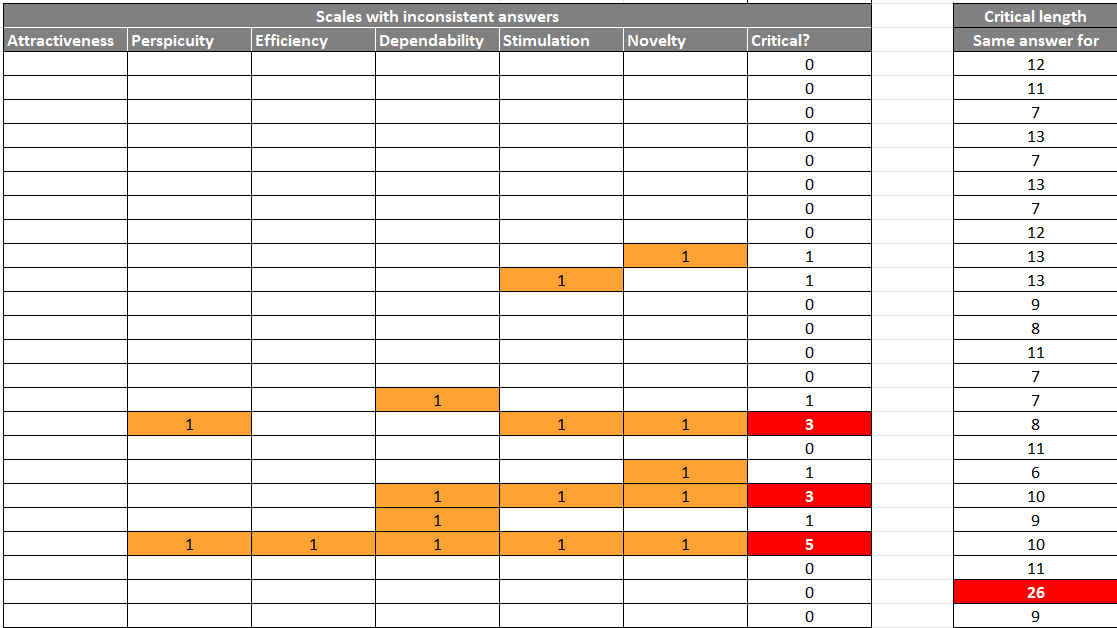
\includegraphics[width=0.8\textwidth]{contents/chapter-4/images/invalidUEQ.png}
	\caption{Data invalid pada UEQ}
	\label{Fig:InvalidUEQ}
\end{figure}

Hasil rata-rata skala UEQ tiap aspek pengalaman pengguna untuk Aplikasi 
MedQ dipaparkan dalam tabel pada gambar \ref*{Fig : Tabel Skor UEQ} dan grafik pada gambar \ref*{Fig : Gambar Skor UEQ }.
\begin{figure}[H]
	\centering
	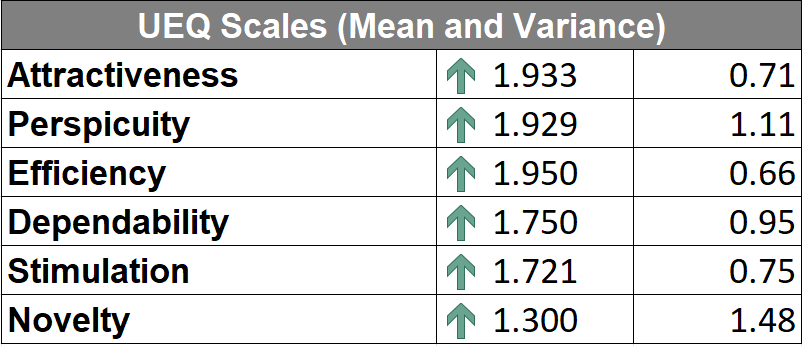
\includegraphics[width=0.6\textwidth]{contents/chapter-4/images/UEQScore.png}
	\caption{Tabel rata-rata hasil pengujian UEQ}
	\label{Fig : Tabel Skor UEQ}
\end{figure}
\begin{figure}[H]
	\centering
	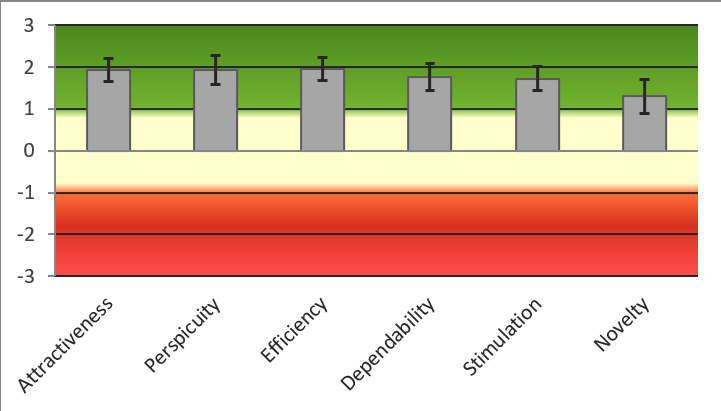
\includegraphics[width=0.7\textwidth]{contents/chapter-4/images/UEQScore-graph.png}
	\caption{Grafik rata-rata hasil pengujian UEQ}
	\label{Fig : Gambar Skor UEQ }
\end{figure}

Aplikasi MedQ mendapat nilai rata-rata 1,93 untuk skala daya tarik atau 
Attractiveness, mendapat nilai rata-rata 1,93 untuk skala kejelasan atau 
Perspicuity dan mendapat nilai ra-rata 1,95 untuk skala efisiensi. Untuk skala 
ketepatan atau \textit{Dependability} aplikasi MedQ mendapat nilai rata-rata 1,75 dan 
mendapat nilai rata-rata 1,72 untuk skala stimulasi. Sedangkan untuk skala 
kebaruan aplikasi MedQ mendapat nilai rata-rata 1,3. 
\begin{figure}[H]
	\centering
	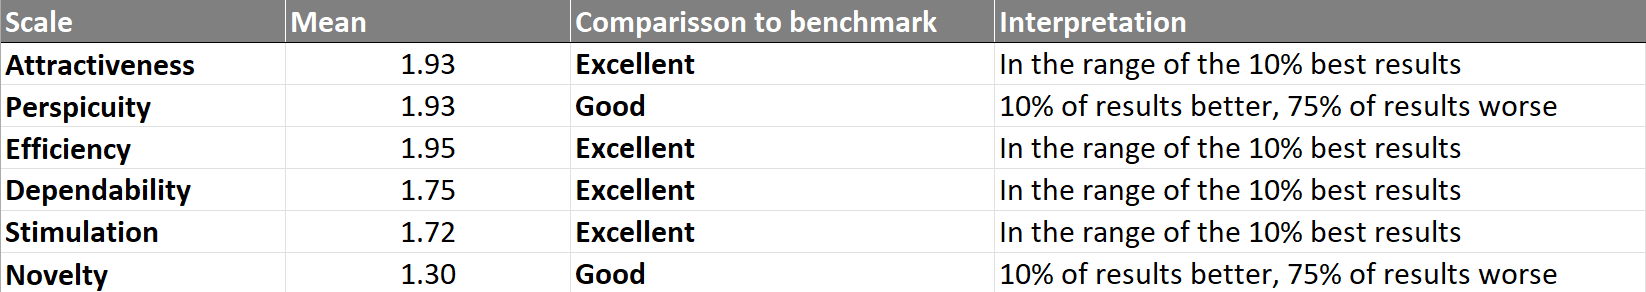
\includegraphics[width=0.9\textwidth]{contents/chapter-4/images/BenchMark.png}
	\caption{Tabel \textit{benchmark} pengujian UEQ}
	\label{Fig : benchmark}
\end{figure}
\begin{figure}[H]
	\centering
	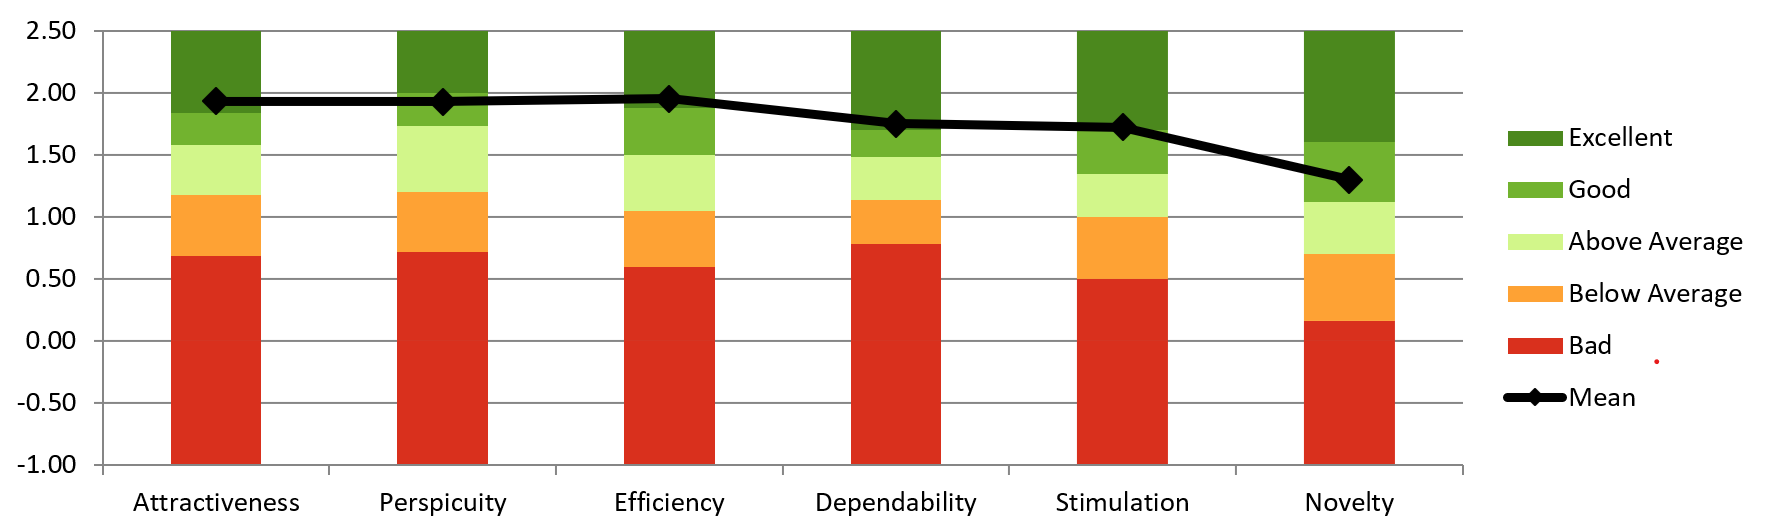
\includegraphics[width=0.8\textwidth]{contents/chapter-4/images/BenchMark-graph.png}
	\caption{Grafik \textit{benchmark} pengujian UEQ}
	\label{Fig : benchmark-graph}
\end{figure}
Apabila dibandingkan dengan benchmark maka aplikasi MedQ masuk ke 
dalam kategori \textit{Excellent} untuk skala daya tarik, efisiensi, ketepatanm dan stimulasi.
Tapi masuk kategori \textit{Good} untuk skala kejelasan dan kebaruan

\newpage
\subsection{Kekurangan Aplikasi}
Aplikasi ini memiliki beberapa kekurangan yang dapat dikembangkan lagi. Kekurangan tersebut diantarannya:
\begin{enumerate}
	\item Aplikasi masih hanya dapat berjalan dalam sistem operasi Android.
	\item Aplikasi masih bisa diimplementasikan fitur tambahan yang dapat memperluas cakupan pengguna aplikasi.
	\item Aplikasi belum memiliki \textit{audio}.
	\item Aplikasi belum memiliki fitur \textit{tutorial} yang dapat membantu pengguna dalam menggunakan aplikasi.
	\item Aplikasi pembelajaran dikembangkan berdasarkan 1 domain pembelajaran.
\end{enumerate}